\documentclass[11pt]{article}
\usepackage[letterpaper,margin=1in]{geometry}
\usepackage{amsmath,amssymb,amsthm,graphicx,booktabs,array,xcolor,hyperref}
\hypersetup{colorlinks=true,linkcolor=blue!45!black,urlcolor=blue!45!black,citecolor=blue!45!black}
\newtheorem{theorem}{Theorem}
\newtheorem{lemma}[theorem]{Lemma}
\newtheorem{proposition}[theorem]{Proposition}
\newtheorem{corollary}[theorem]{Corollary}
\theoremstyle{definition}\newtheorem{definition}[theorem]{Definition}
\setlength{\emergencystretch}{1em}
\setlength{\parskip}{4pt}\setlength{\parindent}{0pt}
\title{A simple orthogonal mirror room with 22 walls}
\author{Peyton Wang\thanks{Investigator, age 16. Peyton led this investigation. Claude/Opus and Codex were used as research and verification tools, including the construction search, separate exact unfolding checks, and independent review of the computer-assisted exclusion. This working note awaits human mathematical review. }}
\date{31 October 2026}
\begin{document}
\maketitle
\begin{abstract}
We give coordinates for a strictly simple orthogonal polygon with 22 maximal straight walls and two distinct interior points that do not illuminate one another. The room comprises three reflected copies of a five-square staircase. A lattice-parity argument and the retracing property of convex right-angle corners give a self-contained proof. We also establish a computer-assisted minimum of 22 within the canonical 45-degree tiling, for two interior A marks and at most four transparent B/C points. Separately, 22 is optimal within a restricted tree-of-copies construction class. Neither lower bound covers general orthogonal rooms.
\end{abstract}

\section{Conventions and construction}
A \emph{wall} is a maximal straight segment of the polygon boundary. A simple room has a single Jordan boundary, with no holes, slits, or boundary point contacts. A billiard path is a finite positive-length polygonal path reflecting specularly at wall interiors; it stops upon reaching an actual polygon corner. A grid point lying inside a straight wall is an ordinary reflecting point, not a corner. A path segment may not lie in a wall. To connect two interior points, the path must reach the target before reaching a corner.

\begin{theorem}\label{thm:room}
Let $Q$ have the following cyclic boundary vertices:
\begin{align*}
&(-1,-1),(0,-1),(0,-2),(1,-2),(1,-3),(2,-3),\\
&(2,-1),(1,-1),(1,1),(3,1),(3,0),(5,0),\\
&(5,1),(4,1),(4,2),(3,2),(3,3),(1,3),\\
&(1,2),(0,2),(0,1),(-1,1).
\end{align*}
Then $Q$ is a simple orthogonal room with 22 walls. The points $S=(0,0)$ and $T=(2,2)$ lie in its interior and are not joined by a billiard path.
\end{theorem}

The coordinates are integers; their absolute scale is immaterial. In particular, the result concerns an ideal point source and target under geometrical optics. It makes no claim about a positive-area dark region or a physical wave cavity.

\begin{figure}[ht]
\centering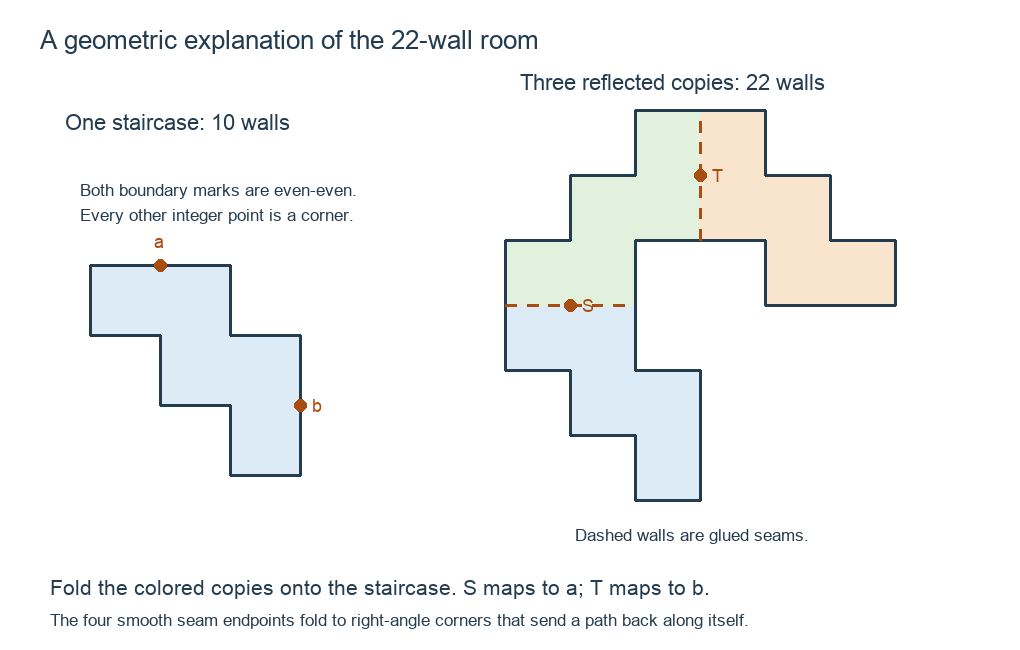
\includegraphics[width=\textwidth]{three-copy-proof.png}
\caption{The five-square base and the three-copy room. Dashed seams are open passages in the room, not reflecting walls. The four seam endpoints are smooth points of the final boundary.}
\label{fig:copies}
\end{figure}

\section{The base obstruction}
Let $P$ be the union of the five closed unit squares with lower-left corners
\[
(-1,-1),\quad(0,-1),\quad(0,-2),\quad(1,-2),\quad(1,-3).
\]
Its two marked smooth boundary points are $a=(0,0)$ and $b=(2,-2)$. The ten genuine corners, in cyclic order, are
\[
(-1,-1),(-1,0),(1,0),(1,-1),(2,-1),(2,-3),
(1,-3),(1,-2),(0,-2),(0,-1).
\]
Directly inspecting the five squares gives the following complete lattice census: seven convex corners, three concave corners, the two smooth points $a,b$, and no interior lattice points. In particular, every integer point in $P$ other than $a,b$ is an actual corner.

\begin{lemma}[Parity]\label{lem:parity}
There is no ordinary billiard path from $a$ to $b$ in $P$.
\end{lemma}
\begin{proof}
Unfold any proposed path by reflecting across the walls it encounters. Each wall lies on an integer horizontal or vertical line. Its reflection preserves integer coordinates and their two parities. The unfolded path is therefore a straight segment from $(0,0)$ to an even-even integer point. Its endpoint is nonzero because the unfolded segment has positive length.

Write that endpoint as $k(p,q)$, where $k>0$ and $p,q$ are coprime integers. Since both endpoint coordinates are even, $k$ is even and at least two. The point $(p,q)$ lies strictly inside the segment and has at least one odd coordinate. Fold that point back along the proposed path. Its image is an integer point of $P$ with at least one odd coordinate, so it is neither $a$ nor $b$. By the census it is an actual corner. The path would encounter that corner before its target, a contradiction.
\end{proof}

No rational-direction assumption is imposed on the initial path. Rationality follows from its integer unfolded endpoint. This distinction is essential: no sampled directions or reflection cutoff are used.

\begin{lemma}[Retracing]\label{lem:retrace}
Allow a path in $P$ to continue at convex right-angle corners by reversing its velocity and retracing its incoming path. Keep concave corners forbidden. This continuation still cannot connect $a$ to $b$.
\end{lemma}
\begin{proof}
Suppose a finite generalized path connects the marks. Restrict it to the portion after its last visit to $a$ and before its first arrival at $b$. If this portion has a corner continuation, consider the first one. It reverses the velocity; reversibility of every preceding ordinary reflection then returns the path to $a$ before reaching any new point. It cannot pass through $b$ on that return, since it did not pass through $b$ on the outward portion. This contradicts the choice of the last visit to $a$. The restricted path therefore has no corner continuation and contradicts Lemma~\ref{lem:parity}.
\end{proof}

Smooth boundary visits, including visits to $a$ or $b$, obey the usual reversible reflection law. For an arriving direction with two nonzero components, continuation through a removable right-angle corner reverses both components. This observation for a convex corner of angle $\pi/2$ is also discussed in Wolecki's Remark~2.2~\cite{wolecki}.

\section{Folding the room onto the base}
Form the three copies
\[
 P_0=P,\qquad P_1=\{(x,-y):(x,y)\in P\},\qquad
 P_2=\{(4-x,-y):(x,y)\in P\}.
\]
The copies satisfy $P_0\subset\{y\le0\}$, $P_1\subset\{y\ge0,x\le2\}$, and $P_2\subset\{y\ge0,x\ge2\}$. These half-plane bounds and the five listed cells show that their interiors are pairwise disjoint. $P_0$ and $P_1$ share exactly the wall $[-1,1]\times\{0\}$; $P_1$ and $P_2$ share exactly $\{2\}\times[1,3]$. There are no other contacts between the copies. Their union is the 15-square room in Theorem~\ref{thm:room}.

Both seam midpoints become interior points: $S=(0,0)$ and $T=(2,2)$. Starting with three ten-wall boundaries, removing the two glued wall pairs subtracts four walls. At each of the four distinct seam endpoints, the two remaining exterior walls are collinear and merge. Thus
\[
 W(Q)=3\cdot10-4-4=22.
\]
The displayed cyclic boundary has no crossings or repeated vertices, and hence establishes simplicity independently of this count.

Fold the copies onto $P$ by
\[
 f_0(x,y)=(x,y),\qquad f_1(x,y)=(x,-y),\qquad
 f_2(x,y)=(4-x,-y).
\]
The maps agree pointwise on each seam. They send $S$ to $a$ and $T$ to $b$. Crossing a seam becomes an ordinary wall reflection downstairs, and an exterior-wall reflection projects to an ordinary reflection except at a seam endpoint.

The four exceptional endpoints are
\[
(-1,0),\quad(1,0),\quad(2,1),\quad(2,3).
\]
Each is smooth upstairs and maps to a convex right-angle corner downstairs. A transverse reflection there switches between the adjacent copies. Composing the reflection in the actual wall with the reflection across the perpendicular seam gives $-I$, so the projected path reverses velocity. These events are precisely the continuations allowed in Lemma~\ref{lem:retrace}. Every preimage of a base corner is either an actual room corner or one of the four seam endpoints. Indeed, the thirty copy-corner incidences are the twenty-two distinct room corners plus two incidences at each seam endpoint. In particular, every preimage of a concave base corner is an actual room corner; a valid path cannot encounter it.

The smooth boundary points $(4,0)$ and $(2,-2)$ are additional preimages of $a$ and $b$. A visit to either projects to an ordinary visit to the corresponding mark. An arrival at $b$ before arrival at $T$ would already give a forbidden path prefix.

An axis-parallel path in $Q$ cannot join $S$ to $T$: horizontal and vertical wall reflections preserve its zero velocity component. All remaining directions have two nonzero components, so seam crossings are transverse and the preceding local analysis applies. A hypothetical $S$--$T$ path therefore projects to a finite generalized $a$--$b$ path in $P$. Lemma~\ref{lem:retrace} excludes it. This proves Theorem~\ref{thm:room}.

\section{A restricted optimality result}\label{sec:restricted}
The following result explains the wall cost of this particular mechanism. It does not classify all dark rooms, all parity proofs, or all reflected-copy constructions.

\begin{definition}
A \emph{parity base} is a simple polyomino $B$ with two distinct smooth boundary lattice marks $a,b$, such that every lattice point of $B$ that is not a genuine polygon corner belongs to $a+2\mathbb Z^2$. Extra smooth or interior lattice points in this residue class are allowed.
\end{definition}
Translation by $a$ reduces this condition to the parity argument in Lemma~\ref{lem:parity}: the first primitive step has a nonzero parity class, and hence folds to an actual corner. Convex-corner retracing remains harmless by Lemma~\ref{lem:retrace}.

\begin{proposition}\label{prop:base}
Every parity base has at least ten maximal walls. The five-square staircase $P$ attains ten.
\end{proposition}
\begin{proof}
Translate $a$ to $(0,0)$. Let $A$ be the number of unit squares and let $c,r$ be the numbers of convex and reflex corners. Call a lattice point \emph{odd} if it does not belong to $2\mathbb Z^2$. Each unit square has exactly three odd vertices. Every occupied odd vertex is an actual polygon corner by hypothesis, so it meets either one square (a convex corner) or three (a reflex corner). Writing $c_o,r_o$ for the odd corner counts gives
\[
 3A=c_o+3r_o\le c+3r=4r+4,
\]
where the last equality uses $c-r=4$.
If the wall count $w=c+r$ is less than ten, then $r\le2$ and $A\le4$.

For completeness, the connected polyominoes with up to four cells are obtained as follows, up to translation, rotation and reflection. With one or two cells there is only the square or domino. With three cells there is a straight strip or an L. With four cells, the cell-adjacency graph either contains a cycle, giving the $2\times2$ square, or is a tree. A degree-three vertex gives the T shape. Otherwise the graph is a four-vertex path. Its three successive unit steps give a straight strip, one turn (the L), two same-sense turns (the excluded square cycle), or two opposite-sense turns (the S). This exhausts the five tetrominoes.

For the table, choose the horizontal strips with lower-left cell coordinates $(j,0)$ for $0\le j<n$, where $n=1,2,3,4$. The L triomino has cells $(0,0),(1,0),(0,1)$; the square tetromino has cells $(0,0),(1,0),(0,1),(1,1)$. The T, L and S tetrominoes use cells $(0,0),(1,0),(2,0),(1,1)$; $(0,0),(1,0),(2,0),(0,1)$; and $(0,0),(1,0),(1,1),(2,1)$. Table~\ref{tab:bases} checks all nine shapes. The square has no smooth boundary marks. Every other shape has non-corner lattice points in at least two residue classes modulo $2\mathbb Z^2$, violating the definition. Integer translations and lattice isometries preserve equality or inequality of these classes. The stated census of $P$ supplies the attaining example.
\end{proof}

\begin{table}[ht]
\centering\small
\begin{tabular}{@{}lrrr@{}}\toprule
Base & Smooth lattice points & Interior lattice points & Non-corner residue classes\\\midrule
Square & 0 & 0 & 0\\
Domino & 2 & 0 & 2\\
Straight triomino & 4 & 0 & 4\\
L triomino & 2 & 0 & 2\\
Straight tetromino & 6 & 0 & 4\\
Square tetromino & 4 & 1 & 3\\
T tetromino & 2 & 0 & 2\\
L tetromino & 4 & 0 & 3\\
S tetromino & 2 & 0 & 2\\\bottomrule
\end{tabular}
\caption{All bases of area at most four. Representatives are specified in the proof; the checker uses the same cells.}\label{tab:bases}
\end{table}

\begin{corollary}\label{cor:restricted}
Consider a construction using $m$ congruent reflected copies of one parity base. Assume their interiors are disjoint, the full-wall seams form a tree with $m-1$ seams, all $2(m-1)$ seam endpoints are distinct, and exactly one straight exterior-wall merge occurs at each endpoint. Assume no other contacts or boundary identifications, and suppose that preimages of both marked base points are interior to the resulting room. Every such room has at least 22 maximal walls. The construction of $Q$ attains this bound with $m=3$.
\end{corollary}
\begin{proof}
Every maximal base wall has integer length at most two. Otherwise it contains two consecutive smooth lattice points, which cannot both belong to $a+2\mathbb Z^2$. Thus any wall contains at most one smooth lattice point. Interior preimages of the two distinct boundary marks require at least two distinct seams: a full-wall seam can interiorize only one of them, and its endpoints remain on the exterior boundary by assumption. Consequently $m\ge3$.

If the base has $w$ walls, removing the $m-1$ glued wall pairs and merging at the $2(m-1)$ distinct endpoints gives
\[
 W=mw-2(m-1)-2(m-1)=m(w-4)+4\ge 3(10-4)+4=22.
\]
Apply Proposition~\ref{prop:base}. The displayed construction attains equality.
\end{proof}

The hypotheses are substantive. Partial-wall gluings, shared seam endpoints, additional contacts, a seam graph with cycles, or a different obstruction are outside the corollary. Extra harmless lattice points are already allowed by the definition of a parity base. Arbitrary orthogonal polygons also need not admit a common unit-square grid.

\section{A bounded canonical-family minimum}

Fix the integer square grid and split each unit square along its A--B diagonal. Here A points have both coordinates even, B points have both coordinates odd, and C points have mixed parity. Every resulting right-isosceles triangle has one vertex of each type. A \emph{transparent B/C point} is a lattice point of type B or C in the room interior or in the relative interior of a straight boundary wall. It remains an ordinary point for billiard motion. The count refers to this fixed presentation, rather than to an invariant of arbitrary subdivisions.

\begin{theorem}[Computer-assisted bounded minimum]\label{thm:bounded}
Let a room be a finite union of triangles of this fixed tiling, with a single strictly simple polygonal boundary and two distinct interior A marks that do not illuminate one another. If it has at most four transparent B/C points, then it has at least 22 maximal straight walls. The room in Theorem~\ref{thm:room} attains equality, with four transparent B/C points.
\end{theorem}

\begin{proof}[Reduction and certificate proof]
Write $N$ for the triangle count, $I$ for the number of interior A points, $J$ for the number of interior B/C points, and $s_A,s_N$ for the smooth boundary A and B/C counts. Put $k=J+s_N$. Let $Q$ count three per smooth boundary A point and one per incident triangle at every genuine boundary A corner. Euler's formula for a triangulated disk and incidence counting give
\[
 W=2+6I+Q-2J-s_N,\qquad N=8I+Q+s_A,\qquad 3s_A\le Q.
\]
The local-fan bound $Q\ge4-s_N$ implies
\[
 W\ge6+6I-2k,\qquad
 N\le\tfrac43(W-2+2k).
\]
Consequently a counterexample with $W\le21$, $k\le4$ must satisfy $2\le I\le3$ and $N\le36$. The local-fan bound and counting details are recorded in the verification bundle described below.

For the finite support reduction, use A-cell coordinates divided by two. Let $F$ be the set of full A cells, let $P$ count occupied partial A cells, and let $R$ contain $F$ and its four-neighbors. Put $b=|R\setminus F|$ and let $m$ count empty cells in $R\setminus F$. Connectedness and the partial-fan charge bound give
\[
 Q\ge2P-2I-2+m,\qquad m\le s_N,\qquad
 2(P+m)\le W-4I+2k.
\]
Indeed, the occupied-cell graph has at least $I+P-1$ edges, full-cell degrees sum to at most $4I-m$, and $Q$ bounds the remaining degrees. Each missing neighboring cell supplies a distinct smooth C point. Combining these observations with the wall identity yields the last inequality.

Even using the conservative threshold $W\le23$, this gives $P+m\le11$ for $I=2$ and $P+m\le9$ for $I=3$. There are at most $P+m-b$ occupied cells outside $R$, so they lie within that Manhattan distance of $R$. For two full cells, symmetry reduces their separation to 14 offsets of Manhattan distance two through six; adjacent marked cells have a direct segment. For three full cells the graph joining full cells at distance at most two is connected, since otherwise $b\ge10$. Rooting one cell at the origin restricts the others to the radius-four diamond. Of 138 connected rooted triples, 120 satisfy $b\le9$, giving eight shapes up to grid isometries and translation. Their nonadjacent marked pairs give 17 cases. Thus 22 supports and 31 marked-pair cases cover every counterexample.

For each case an independently written Boolean formula imposes necessary conditions: legal single-sector local fans, the exact full-A set, $N\le36$, $W\le21$, $k\le4$, the disk turning identity, and connectivity. Previously checked connecting-path certificates forbid their sufficient lighting premises. Every eligible dark room therefore induces a satisfying assignment.

All 31 formulas are unsatisfiable. CaDiCaL 1.9.5 produced a DRAT contradiction trace for each; a separate \texttt{drat-trim} verifier accepted every trace. All final formulas regenerate byte for byte from the frozen reviewed encoder and inputs, and all adopted traces passed an additional independent replay. No case uses optional component cuts. Hence no eligible counterexample exists. The already certified room supplies equality.
\end{proof}

\paragraph{Evidence and trust boundary.}
The local verification bundle is \path{bounded-proof/}, relative to this note. The files \path{support-proof.md} and \path{encoding-proof.md} state the necessary geometric implications; \path{proof-manifest.json} lists all 31 formula/trace hashes. Frozen reviewed source, support data, path inputs and regeneration records are under \path{provenance/}; \path{provenance-repair.json} records 31 byte-exact reconstructions and 31 fresh DRAT checks. The final formulas contain 2,692,369 clauses in total. These are Boolean artifact counts, not room or ray counts.

The static witness audit in \path{persisted-replay/} checked 34,897 precomputed and 12,679 learned records using exact arithmetic. No new billiard rays were searched for this proof. Claude/Opus reviewed the necessary encoding and support reductions independently; Codex independently reproduced the formulas and checked the adopted proofs. This is a computer-assisted theorem whose written geometric reductions and software still require mathematical review, rather than a fully formalized geometry proof.

The restriction $k\le4$ is essential to this result. It does not establish the minimum for $k\ge5$, for arbitrary marked points, or for rooms outside the fixed canonical tiling. In particular it does not assert a global minimum of 22.

\section{Verification, prior work, and the open bound}
The cell and seam identities, lattice census, wall count, and corner fibers are checked using exact integer arithmetic in \texttt{geometric-proof-check.py}. The saved UTF-8 JSON input file \texttt{peer-fast-inputs/cand-2\_2-1.json} has SHA-256
\begin{center}\scriptsize\ttfamily
c7838dfe640932458e6853af7171396af05df71067658ee8f78f9ca3d91cab20.
\end{center}
A separate finite proof reconstructs the physical four-orientation unfolding as 60 squares and supplies a closed set of 2,592 labelled states under the elementary integral shears and their inverses. An independent readback verifies 10,368 closure transitions and 10,368 horizontal source-sector checks, with no connecting path. These counts concern the physical unfolding. A separate 20-square quotient has a 72-state certificate; it is not needed for the hand proof above. Neither proof samples rays or imposes a reflection bound. The small-base table is checked by \texttt{lower-bound-check.py}, which only evaluates the explicitly listed shapes.

Related polygonal constructions appear in Tokarsky~\cite{tokarsky}, Castro~\cite{castro}, Tokarsky--Boese~\cite{boese}, and Wolecki~\cite{wolecki}.

An exact reconstruction of Wolecki's published vector figure finds a point contact in its boundary. O'Rourke's public orthogonal example~\cite{orourke} has 34 walls. The coordinate checks distinguish these specific displayed polygons.

For a general simple orthogonal room let $r$ and $c$ be the numbers of reflex and convex corners. Turning angle gives $c-r=4$, hence
\[
 W=c+r=2r+4.
\]
Our room has $r=9$ and $c=13$. A global lower bound of 22 would require showing that every such room with $r\le8$ connects every pair of distinct interior points. Nothing in Corollary~\ref{cor:restricted} supplies that assertion.

Moreover, wall count cannot bound area, side-length ratios, or the number of lattice exceptions in an arbitrary chosen subdivision. Integer dilation preserves wall count and darkness while increasing subdivision complexity. Even fixing a primitive grid does not by itself give a finite bound on side-length ratios. A complete lower bound must therefore use an invariant of the room and its reflected paths, or a justified reduction covering all lengths and marked points. Establishing such a reduction is the next open problem.

\clearpage
\begin{thebibliography}{9}\small
\bibitem{tokarsky} G. W. Tokarsky, \emph{Polygonal Rooms Not Illuminable from Every Point}, Amer. Math. Monthly 102(10) (1995), 867--879. \href{https://doi.org/10.1080/00029890.1995.12004679}{doi:10.1080/00029890.1995.12004679}. Original full text was not recovered in this audit; attribution is corroborated by later primary accounts.
\bibitem{castro} D. Castro, reader letter, \emph{Quantum} 7(3) (January/February 1997), 42. \href{https://static.nsta.org/pdfs/QuantumV7N3.pdf\#page=44}{Original letter}.
\bibitem{boese} G. W. Tokarsky and F. G. Boese, \emph{Invisible Points in a House of Mirrors}, Mathematics Magazine 73(5) (2000), 364--369. \href{https://doi.org/10.1080/0025570X.2000.11996877}{doi:10.1080/0025570X.2000.11996877}. Relevant text checked in a public scan; original figure comparison remains incomplete.
\bibitem{wolecki} A. Wolecki, \emph{Illumination in Rational Billiards}, arXiv:1905.09358, v1 (2019), v3 (30 November 2024). \url{https://arxiv.org/html/1905.09358v3}.
\bibitem{orourke} J. O'Rourke, \emph{Art Gallery Visibility Theorems: An Introduction}, author page and public Fig.9.14, forthcoming-book materials labelled 2026/2027. \url{https://www.science.smith.edu/~jorourke/AGVT/}.
\end{thebibliography}
\end{document}
